% Provenance (never printed): see sources/outline_sources.md (Year 3: the heat
% equation, half-space and plate cooling models, heat flow against age,
% continental geotherms, thermal subsidence). Brief: sources/book5/BRIEFS.md,
% ch. 5. Curves from figdata/bachelor-3/plate_cooling.py (models; Seton et al.
% 2020 age grid and ETOPO1, read only) and continental_geotherm.py.
% Exercise and problem values in the Book 5 scratch calculator calc/ch05.py.
\chapter{Thermal Models of the Lithosphere}\label{ch:b3:lithosphere-thermal-models}

Sail away from a mid-ocean ridge and the sea floor deepens: about
\qty{2.5}{km} at the axis, more than \qty{5}{km} beneath the oldest ocean
floor. Nothing has been added to the plate or taken away from it; it has only
cooled, contracted and sunk. The ocean floor is a thermometer of the plate
beneath it, and a heat-flow probe pushed into its sediment reads the same
cooling from above. This chapter solves the cooling of a plate in two ways, as
a half-space and as a plate of finite thickness, compares both with the depth
of the real ocean floor and its heat flow, and then turns to the continents,
whose heat comes partly from their own crust.
% ledger: ps77:depth-age

\begin{recall}
The diffusion equation for heat, $\partial T/\partial t = \kappa\nabla^2T$,
with the thermal conductivity $k$ and the thermal diffusivity $\kappa =
k/(\rho c)$, is the physics books'; Fourier series and the error function
$\operatorname{erf}x = (2/\sqrt\pi)\int_0^xe^{-u^2}\,\mathrm du$ are in the
mathematics books' university volumes. The heat flow, the radiogenic heat
production, the geotherm, the conductive time scale $L^2/\kappa$, the thermal
boundary layer and the thermal lithosphere were defined in the Year 1 volume,
in its chapter on the Earth's heat budget; isostasy in its chapter on isostasy
and gravity anomalies; the depth--age law $d = d_r + C\sqrt t$ was proved in
its chapter on rifts, ridges and passive margins, admitting the temperature
profile that this chapter derives. The stretching model of basins, post-rift
subsidence and the thermal time constant are in the Year 2 volume, in its
chapter on sedimentary basins.
\end{recall}

\section{Conduction, advection and their ratio}

Heat in the lithosphere moves in two ways: it diffuses down the temperature
gradient, and it is carried by moving rock, the plate leaving a ridge, an
eroded mountain rising, a magma ascending. Which one wins depends on a single
number.

\begin{definition}[Thermal Péclet number]\label{def:b3:lithosphere-thermal-models:peclet}
For rock moving at the speed $u$ across a length $L$, the \emph{thermal Péclet
number}\index{thermal Péclet number} is
\[
  \mathrm{Pe} = \frac{uL}{\kappa},
\]
the ratio of the conductive time $L^2/\kappa$ to the advective time $L/u$.
Advection dominates where $\mathrm{Pe} \gg 1$, conduction where
$\mathrm{Pe} \ll 1$.
\end{definition}

A plate leaving a ridge at \qty{25}{mm/yr} has, over a distance of
\qty{95}{km}, $\mathrm{Pe} \approx 94$ with $\kappa = \qty{0.8e-6}{m^2.s^{-1}}$:
heat is carried sideways by the plate far faster than it diffuses sideways.
Each vertical column of the plate therefore cools as if alone, by vertical
conduction to the cold sea floor, its age $t$ standing for the time since it
left the axis. That turns a problem in two dimensions into one in depth and
time.

\section{The cooling half-space}

\begin{definition}[Half-space cooling model]\label{def:b3:lithosphere-thermal-models:half-space}
The \emph{half-space cooling model}\index{half-space cooling model} of the
oceanic lithosphere takes each column as a half-space $z \ge 0$ of uniform
diffusivity, at the uniform temperature $T_m$ of the mantle when it leaves the
ridge axis, whose surface is held from then on at the temperature $T_0$ of the
sea floor, with no heat production and no bottom.
\end{definition}

\begin{theorem}[Error-function geotherm]\label{thm:b3:lithosphere-thermal-models:erf}
In the \omterm{def:b3:lithosphere-thermal-models:half-space}{half-space cooling model}, the temperature at the depth $z$ below the
sea floor of age $t$ is
\[
  T(z, t) = T_0 + (T_m - T_0)\operatorname{erf}\frac{z}{2\sqrt{\kappa t}} .
\]
This is the \emph{error-function geotherm}\index{error-function geotherm}.
\end{theorem}

\begin{proof}
Let $\theta = (T - T_0)/(T_m - T_0)$; it solves $\partial\theta/\partial t =
\kappa\,\partial^2\theta/\partial z^2$ with $\theta(z, 0) = 1$ for $z > 0$ and
$\theta(0, t) = 0$ for $t > 0$. The problem has no length scale of its own:
if $\theta(z, t)$ is a solution, so is $\theta(\lambda z, \lambda^2t)$ for every
$\lambda > 0$, with the same initial and boundary values; the solution being
unique, $\theta$ depends on $z$ and $t$ only through $\eta = z/(2\sqrt{\kappa
t})$. Writing $\theta = f(\eta)$, with $\partial\eta/\partial t = -\eta/(2t)$ and
$\partial\eta/\partial z = 1/(2\sqrt{\kappa t})$,
\[
  -\frac{\eta}{2t}f'(\eta) = \kappa\,\frac{f''(\eta)}{4\kappa t},
  \qquad\text{so}\qquad f'' + 2\eta f' = 0 .
\]
Hence $f' = Ae^{-\eta^2}$ and $f = A\int_0^\eta e^{-u^2}\,\mathrm du + B$. The
surface condition, at $\eta = 0$, gives $B = 0$; the initial condition, which
holds at every depth as $t \to 0$, that is as $\eta \to \infty$, gives
$A\sqrt\pi/2 = 1$. So $f = \operatorname{erf}\eta$.
\end{proof}

The temperature at a given depth depends only on $z/\sqrt t$: an isotherm sinks
as the square root of age, and the cooled layer at \qty{40}{Myr} is twice as
thick as at \qty{10}{Myr}. The surface heat flow follows by differentiation.

\begin{proposition}[Heat flow--age relation]\label{prop:b3:lithosphere-thermal-models:heat-flow}
In the \omterm{def:b3:lithosphere-thermal-models:half-space}{half-space cooling model}, the heat flow through the sea floor of age $t$
is
\[
  q(t) = k\,\frac{\partial T}{\partial z}\Big|_{z=0}
  = \frac{k(T_m - T_0)}{\sqrt{\pi\kappa t}} = \frac{C_q}{\sqrt t} .
\]
\end{proposition}

\begin{proof}
$\partial\operatorname{erf}(z/2\sqrt{\kappa t})/\partial z = (2/\sqrt\pi)
e^{-z^2/4\kappa t}/(2\sqrt{\kappa t})$, which at $z = 0$ is $1/\sqrt{\pi\kappa
t}$.
\end{proof}

With the values of the plate model below ($k = \qty{3.1}{W.m^{-1}.K^{-1}}$,
$T_m - T_0 = \qty{1450}{K}$, $\kappa = \qty{0.8e-6}{m^2.s^{-1}}$), $C_q =
\qty{505}{mW.m^{-2}.Myr^{1/2}}$, close to the values of 430 to
\qty{510}{mW.m^{-2}.Myr^{1/2}} fitted to the global measurements by different
studies; a recent compilation prefers \num{490}. Measured heat flow on young
oceanic crust, however, grossly underestimates the heat that leaves it:
sea water circulating through the cracked crust carries part of the heat away
in hot springs, out of reach of the probes. Over old crust the measurements
follow $1/\sqrt t$, and estimates of the Earth's heat loss replace the
measurements on crust younger than \qty{66.5}{Myr} with $C_q/\sqrt t$.
% ledger: honda04:gdh1, b2dd10:half-space, dd10b5:hydrothermal

The Year 1 volume integrated the same profile over depth, through isostasy, to
obtain the depth--age law, $d = d_r + C\sqrt t$ with $C = 2\rho_m\alpha(T_m -
T_0)\sqrt\kappa/\bigl(\sqrt\pi(\rho_m - \rho_w)\bigr)$ (figure below). With
$\rho_m = \qty{3300}{kg.m^{-3}}$, $\rho_w = \qty{1030}{kg.m^{-3}}$ and $\alpha =
\qty{3.1e-5}{K^{-1}}$, $C = \qty{370}{m.Myr^{-1/2}}$, against the
\qty{350}{m.Myr^{-1/2}} fitted to the North Pacific and North Atlantic floors
younger than \qty{70}{Myr}.
% ledger: ps77:depth-age

\begin{omfigure}
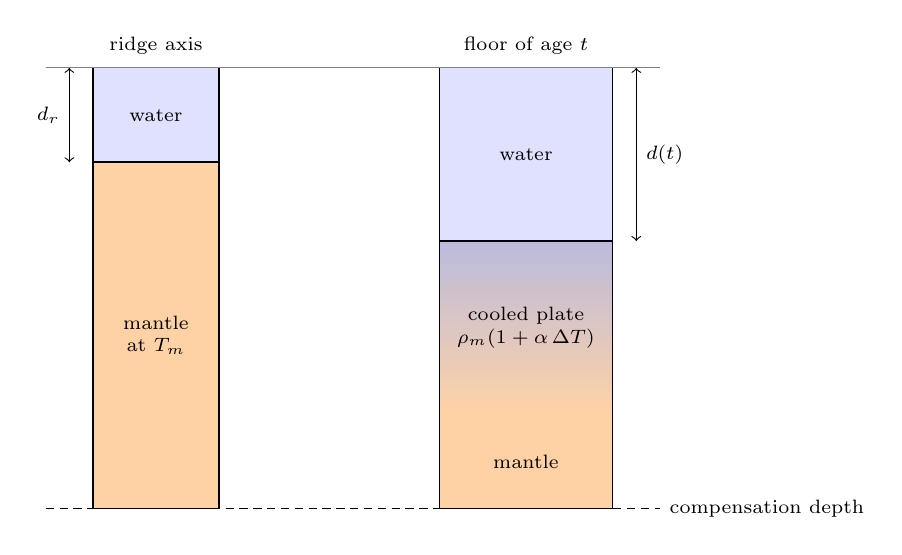
\begin{tikzpicture}[font=\small, x=1cm, y=1cm]
% schematic: two columns of equal mass above the compensation depth
\fill[blue!12] (0,0) rectangle (1.6,-1.2);
\fill[orange!35] (0,-1.2) rectangle (1.6,-5.6);
\fill[blue!12] (4.4,0) rectangle (6.6,-2.2);
\shade[top color=blue!35!gray!40, bottom color=orange!35] (4.4,-2.2) rectangle (6.6,-4.4);
\fill[orange!35] (4.4,-4.4) rectangle (6.6,-5.6);
\draw (0,0) rectangle (1.6,-5.6) (4.4,0) rectangle (6.6,-5.6);
\draw[densely dashed] (-0.6,-5.6) -- (7.2,-5.6) node[right, font=\scriptsize] {compensation depth};
\draw[thick] (0,-1.2) -- (1.6,-1.2) (4.4,-2.2) -- (6.6,-2.2);
\node[font=\scriptsize] at (0.8,-0.6) {water};
\node[font=\scriptsize, align=center] at (0.8,-3.4) {mantle\\at $T_m$};
\node[font=\scriptsize] at (5.5,-1.1) {water};
\node[font=\scriptsize, align=center] at (5.5,-3.3) {cooled plate\\$\rho_m(1 + \alpha\,\Delta T)$};
\node[font=\scriptsize, align=center] at (5.5,-5.0) {mantle};
\draw[<->] (-0.3,0) -- (-0.3,-1.2) node[midway, left, font=\scriptsize] {$d_r$};
\draw[<->] (6.9,0) -- (6.9,-2.2) node[midway, right, font=\scriptsize] {$d(t)$};
\node[above, font=\scriptsize] at (0.8,0.05) {ridge axis};
\node[above, font=\scriptsize] at (5.5,0.05) {floor of age $t$};
\draw[gray] (-0.6,0) -- (7.2,0);
\end{tikzpicture}

\par\smallskip{\small Isostasy of the cooling plate: the column at the ridge
and the column of age $t$ have the same mass above the compensation depth. The
cooled, denser plate sinks, and water fills the space above
it.}\label{fig:b3:lithosphere-thermal-models:columns}
\end{omfigure}

\section{The plate model}

Old ocean floor stops deepening: in the North Pacific and North Atlantic the
depth departs from $\sqrt t$ between 60 and \qty{80}{Myr}, and heat flow levels
off. The half-space keeps cooling for ever; something must hold the base of the
plate warm.
% ledger: parsons:plate-model

\begin{definition}[Plate cooling model]\label{def:b3:lithosphere-thermal-models:plate}
The \emph{plate cooling model}\index{plate cooling model} of the oceanic
lithosphere takes each column as a layer $0 \le z \le L$ of uniform
diffusivity, at the uniform temperature $T_m$ when it leaves the ridge, whose
surface is held at $T_0$ and whose base is held at $T_m$ from then on.
\end{definition}

\begin{theorem}[Plate-model temperature series]\label{thm:b3:lithosphere-thermal-models:plate-series}
In the \omterm{def:b3:lithosphere-thermal-models:plate}{plate cooling model}, with $T_0 = 0$,
\[
  T(z, t) = T_m\Bigl[\frac zL + \frac2\pi\sum_{n=1}^\infty\frac1n
  \sin\frac{n\pi z}{L}\,e^{-n^2t/\tau}\Bigr],\qquad
  \tau = \frac{L^2}{\pi^2\kappa} .
\]
This is the \emph{plate-model temperature series}\index{plate-model temperature series}.
\end{theorem}

\begin{proof}
The steady state, reached as $t \to \infty$, is the linear profile $T_mz/L$.
The departure $u = T - T_mz/L$ solves the diffusion equation with $u = 0$ at
$z = 0$ and $z = L$, and starts as $u(z, 0) = T_m(1 - z/L)$. Separating the
variables, $u = Z(z)\Theta(t)$ gives $Z''/Z = \Theta'/(\kappa\Theta) = -\mu^2$;
the boundary conditions leave $Z = \sin(n\pi z/L)$, $\mu = n\pi/L$, and
$\Theta = e^{-n^2\pi^2\kappa t/L^2} = e^{-n^2t/\tau}$. The initial values fix the
coefficients $b_n$ of the sine series of $T_m(1 - z/L)$ on $[0, L]$:
\[
  b_n = \frac2L\int_0^LT_m\Bigl(1 - \frac zL\Bigr)\sin\frac{n\pi z}{L}\,\mathrm dz
  = \frac{2T_m}{n\pi},
\]
by an integration by parts. Summing the modes gives the series.
\end{proof}

Each mode decays with its own time, $\tau/n^2$: the higher harmonics, the fine
structure of the initial step, vanish first, and after a time of order $\tau$
only the first one is left. The same separation of variables gives the heat
flow and, through the isostatic balance of the figure above, the depth.

\begin{proposition}[Depth and heat flow of the plate model]\label{prop:b3:lithosphere-thermal-models:plate-depth}
In the \omterm{def:b3:lithosphere-thermal-models:plate}{plate cooling model}, with the densities and expansion of the depth--age
law,
\[
  q(t) = \frac{kT_m}{L}\Bigl[1 + 2\sum_{n=1}^\infty e^{-n^2t/\tau}\Bigr],\qquad
  d(t) = d_r + \frac{\rho_m\alpha T_mL}{2(\rho_m - \rho_w)}
  \Bigl[1 - \frac{8}{\pi^2}\sum_{n\ \text{odd}}\frac{e^{-n^2t/\tau}}{n^2}\Bigr].
\]
As $t \to \infty$, the depth tends to $d_r + \rho_m\alpha T_mL/\bigl(2(\rho_m -
\rho_w)\bigr)$ and the heat flow to $kT_m/L$, both exponentially, with the time
constant $\tau$.
\end{proposition}

\begin{proof}
Differentiating the series at $z = 0$, $\partial T/\partial z = (T_m/L)[1 +
2\sum e^{-n^2t/\tau}]$. For the depth, the isostatic balance gives $(\rho_m -
\rho_w)(d - d_r) = \rho_m\alpha\int_0^L(T_m - T)\,\mathrm dz$. The linear part
contributes $T_mL/2$; each mode contributes $-(2T_m/n\pi)e^{-n^2t/\tau}
\int_0^L\sin(n\pi z/L)\,\mathrm dz = -(2T_m/n\pi)(L/n\pi)(1 - \cos n\pi)
e^{-n^2t/\tau}$, which is zero for even $n$ and $-(4T_mL/n^2\pi^2)
e^{-n^2t/\tau}$ for odd $n$. Factoring $T_mL/2$ gives the bracket. At $t = 0$
it vanishes, since $\sum_{n\ \text{odd}}1/n^2 = \pi^2/8$.
\end{proof}

The plate model that best fits the global depths and heat flows has a plate
\qty{95}{km} thick with a base at \qty{1450}{\celsius}, $\alpha =
\qty{3.1e-5}{K^{-1}}$ and $k = \qty{3.1}{W.m^{-1}.K^{-1}}$, thinner and hotter
than the earlier \qty{125}{km} and \qty{1350}{\celsius}. With $\kappa =
\qty{0.8e-6}{m^2.s^{-1}}$, $\tau = \qty{36.2}{Myr}$; the depth levels off at
$2500 + 3104 = \qty{5604}{m}$ and the heat flow at \qty{47}{mW.m^{-2}}. Young
floor cannot tell the two models apart: they differ by less than a metre at
\qty{2}{Myr}, by \qty{100}{m} at \qty{44}{Myr}. Seismology gives a similar
answer: Pacific \omterm{def:b3:seismology-imaging:surface-waves}{Rayleigh waves} are best fitted by cooling plates whose
asymptotic thickness is 85 to \qty{95}{km}.
% ledger: honda04:gdh1, ps77:depth-age, fischer:lithosphere

\begin{omfigure}
\begin{tikzpicture}
\begin{groupplot}[group style={group size=1 by 2, vertical sep=2.3cm},
  omrecord, width=0.86\linewidth, height=0.42\linewidth, xmin=0, xmax=160,
  xlabel={age of the sea floor (Myr)}]
\nextgroupplot[omdepth, ylabel={depth (km)}, ymin=0, ymax=130,
  title={(a) isotherms, every \qty{200}{\celsius}}, title style={font=\small},
  legend style={font=\scriptsize, at={(0.01,0.03)}, anchor=south west}]
% computed in figdata/bachelor-3/plate_cooling.py; ledger: honda04:gdh1
\addplot[omDef, thick] table[x=t, y=hs200] {figdata/out/bachelor-3-plate_cooling-isotherms.dat};
\addlegendentry{half-space}
\addplot[red!70!black, thick, densely dashed] table[x=t, y=pl200] {figdata/out/bachelor-3-plate_cooling-isotherms.dat};
\addlegendentry{plate, $L = \qty{95}{km}$}
\foreach \lev in {400,600,800,1000,1200,1400} {
  \addplot[omDef, thick, forget plot] table[x=t, y=hs\lev] {figdata/out/bachelor-3-plate_cooling-isotherms.dat};
  \addplot[red!70!black, thick, densely dashed, forget plot] table[x=t, y=pl\lev] {figdata/out/bachelor-3-plate_cooling-isotherms.dat};
}
\draw[gray] (axis cs:0,95) -- (axis cs:160,95);
\node[font=\scriptsize, anchor=north] at (axis cs:68,96) {base of the plate};
\node[font=\scriptsize, fill=white, inner sep=1pt] at (axis cs:150,14) {200};
\node[font=\scriptsize, fill=white, inner sep=1pt] at (axis cs:28,38.2) {1000};
\node[font=\scriptsize, fill=white, inner sep=1pt] at (axis cs:22,70.4) {1400};
\nextgroupplot[ylabel={heat flow (\unit{mW.m^{-2}})}, ymin=0, ymax=300,
  title={(b) heat flow}, title style={font=\small},
  legend style={font=\scriptsize, at={(0.98,0.97)}, anchor=north east}]
\addplot[omDef, thick] table[x=t, y=hs] {figdata/out/bachelor-3-plate_cooling-heat.dat};
\addlegendentry{half-space}
\addplot[red!70!black, thick, densely dashed] table[x=t, y=pl] {figdata/out/bachelor-3-plate_cooling-heat.dat};
\addlegendentry{plate}
\end{groupplot}
\end{tikzpicture}

\par\smallskip{\small The two cooling models with the parameters of the text.
(a) Depth of the isotherms from \qty{200}{\celsius} (top) to
\qty{1400}{\celsius} (bottom): those of the half-space go on sinking as
$\sqrt t$, those of the plate stop as the profile becomes linear. (b) Surface
heat flow: the plate model levels off at \qty{47}{mW.m^{-2}}, the half-space
falls as $1/\sqrt t$.}\label{fig:b3:lithosphere-thermal-models:isotherms}
\end{omfigure}

The real ocean floor can be put on the same graph (figure below). Every cell of
one degree of latitude and longitude whose age is known is placed at its age and
its depth; the median of each five-million-year bin rises with age as the models
say for the first \qty{40}{Myr}, but the observed floor is shallower than both
models, and more and more so with age. Nothing has been corrected: old floor
carries a thicker blanket of sediment, more than a kilometre in the older North
Atlantic, which loads it and raises its top, and old floor has had time to
collect seamounts, volcanic plateaus and the swells of hotspots. The published
fits remove the sediment load and the obvious swells first; the depth--age
law of the Year 1 volume, and the plate models above, come from such corrected
depths.
% ledger: data:b5-depth-age, ps77:depth-age

\begin{omfigure}
\begin{tikzpicture}
\begin{axis}[omrecord, omdepth, width=0.86\linewidth, height=0.5\linewidth,
  xmin=0, xmax=180, ymin=2, ymax=6.5, xlabel={age of the sea floor (Myr)},
  ylabel={depth (km)},
  legend style={font=\scriptsize, at={(0.5,-0.24)}, anchor=north, cells={anchor=west}},
  legend columns=2]
% computed in figdata/bachelor-3/plate_cooling.py; ledger: data:b5-depth-age, honda04:gdh1
\addplot[only marks, mark=*, mark size=1.3pt, black,
  error bars/.cd, y dir=both, y explicit]
  table[x=t, y expr=\thisrow{med}/1000, y error plus expr=(\thisrow{q3}-\thisrow{med})/1000,
  y error minus expr=(\thisrow{med}-\thisrow{q1})/1000] {figdata/out/bachelor-3-plate_cooling-bins.dat};
\addlegendentry{observed, median and quartiles}
\addplot[omDef, thick] table[x=t, y expr=\thisrow{hs}/1000] {figdata/out/bachelor-3-plate_cooling-depth.dat};
\addlegendentry{half-space}
\addplot[red!70!black, thick, densely dashed] table[x=t, y expr=\thisrow{pl}/1000] {figdata/out/bachelor-3-plate_cooling-depth.dat};
\addlegendentry{plate, $L = \qty{95}{km}$}
\end{axis}
\end{tikzpicture}

\par\smallskip{\small Depth of the ocean floor against its age: the median and
the quartiles of the depths of the one-degree cells of each five-million-year
bin (sea floor deeper than \qty{1000}{m}, ages from a global age grid, depths
from a global relief model, no correction for sediment, seamounts or swells),
with the two cooling models of the text.}\label{fig:b3:lithosphere-thermal-models:depth-age}
\end{omfigure}

\begin{definition}[Thermal subsidence]\label{def:b3:lithosphere-thermal-models:thermal-subsidence}
\emph{Thermal subsidence}\index{thermal subsidence} is the sinking of the
surface of the lithosphere as it cools and contracts towards thermal
equilibrium, the space above it being filled by water or sediment; isostasy
converts the heat lost by a column into its sinking.
\end{definition}

The ocean floor is the pure case. A stretched continental basin is another: a
lithosphere thinned by a factor $\beta$ brings hot asthenosphere up, and the
post-rift subsidence of the Year 2 volume is the same plate cooling, starting
from a different profile, with the same modes and the same decay times $\tau/n^2$.
Keeping only the first mode is therefore a good approximation once the higher
ones have died away, and a poor one before: for the ocean floor of the plate
model above, the first term alone gives the depth to within two metres after
\qty{20}{Myr}, but is \qty{84}{m} too deep at \qty{5}{Myr}.

\section{Continental geotherms}

Continental crust makes heat: granite carries uranium, thorium and potassium in
concentrations that make the heat produced in the upper crust a large part of
the heat flow at the surface. How the production is distributed with depth
decides the temperature at depth.

\begin{definition}[Heat-production depth scale; reduced heat flow]\label{def:b3:lithosphere-thermal-models:reduced}
When the radiogenic heat production of the crust decreases with depth as
$A(z) = A_0e^{-z/h_r}$, $h_r$ is the \emph{heat-production depth
scale}\index{heat-production depth scale}. The \emph{reduced heat
flow}\index{reduced heat flow} $q_m$ of a province is the heat flow that would
remain at its surface if the crust produced no heat: the heat flow from below
the radiogenic layer.
\end{definition}

\begin{proposition}[Exponential heat production]\label{prop:b3:lithosphere-thermal-models:exponential}
In steady conduction with uniform conductivity $k$, surface temperature $0$,
heat production $A_0e^{-z/h_r}$ and heat flow $q_m$ from great depth, the
surface heat flow is
\[
  q_0 = q_m + A_0h_r,
\]
and the geotherm is
\[
  T(z) = \frac{q_mz}{k} + \frac{A_0h_r^2}{k}\bigl(1 - e^{-z/h_r}\bigr).
\]
If the plutons of a province share the same $h_r$ and the same $q_m$, their
surface heat flows and surface heat productions lie on the straight line
$q_0 = q_m + h_rA_0$.
\end{proposition}

\begin{proof}
In steady state the upward heat flow $q(z) = k\,\mathrm dT/\mathrm dz$ decreases
upwards by the heat produced: $\mathrm dq/\mathrm dz = -A(z)$. With $q \to q_m$
at depth, $q(z) = q_m + A_0h_re^{-z/h_r}$, so $q_0 = q_m + A_0h_r$. Integrating
$\mathrm dT/\mathrm dz = q(z)/k$ from $T(0) = 0$ gives the geotherm. The last
statement is the first one, read for each pluton.
\end{proof}

The line is observed: in several provinces, the heat flows and the surface heat
productions of plutons fall on straight lines, with depth scales of 7.5 to
\qty{10}{km} and a \omterm{def:b3:lithosphere-thermal-models:reduced}{reduced heat flow} of \qty{0.8}{HFU} (about
\qty{33.5}{mW.m^{-2}}) east of the Rocky Mountains. The exponential form is not
the only one that gives a line, but it keeps the line through erosion: removing a slice of thickness $e$ from the top multiplies
$A_0$ and the radiogenic part of $q_0$ by the same factor $e^{-e/h_r}$.
% ledger: b2roy:provinces

The figure below shows geotherms for surface heat flows of 40, 60 and
\qty{80}{mW.m^{-2}}, the first typical of cratons and the last of back-arc
regions, with $k = \qty{2.5}{W.m^{-1}.K^{-1}}$, $h_r = \qty{10}{km}$ and a
crustal share $A_0h_r = 0.4\,q_0$. The \qty{1300}{\celsius} isotherm, taken as
the base of the thermal lithosphere, lies at 129, 84 and \qty{61}{km}.
Seismology finds cratonic mantle fast down to about \qty{250}{km}, and back-arc
lithosphere 50 to \qty{60}{km} thick: the cold, thick roots of cratons need a
smaller \omterm{def:b3:lithosphere-thermal-models:reduced}{reduced heat flow} than this simple model gives them, and their
conductivity changes with temperature, but the order of the contrast is right.
% ledger: hyndman:backarc, fischer:lithosphere, delaney86:properties

\begin{omfigure}
\begin{tikzpicture}
\begin{axis}[omrecord, omdepth, width=0.62\linewidth, height=0.6\linewidth,
  xmin=0, xmax=1600, ymin=0, ymax=200, xlabel={temperature (\unit{\celsius})},
  ylabel={depth (km)},
  legend style={font=\scriptsize, at={(0.02,0.03)}, anchor=south west, cells={anchor=west}}]
% computed in figdata/bachelor-3/continental_geotherm.py
\addplot[black, thick] table[x=T40, y=z] {figdata/out/bachelor-3-continental_geotherm-geotherms.dat};
\addlegendentry{$q_0 = \qty{40}{mW.m^{-2}}$}
\addplot[omDef, thick, densely dashed] table[x=T60, y=z] {figdata/out/bachelor-3-continental_geotherm-geotherms.dat};
\addlegendentry{$q_0 = \qty{60}{mW.m^{-2}}$}
\addplot[red!70!black, thick, dashdotted] table[x=T80, y=z] {figdata/out/bachelor-3-continental_geotherm-geotherms.dat};
\addlegendentry{$q_0 = \qty{80}{mW.m^{-2}}$}
\draw[gray, densely dotted] (axis cs:1300,0) -- (axis cs:1300,200);
\node[font=\scriptsize, rotate=90, anchor=south] at (axis cs:1300,160) {\qty{1300}{\celsius}};
\end{axis}
\end{tikzpicture}

\par\smallskip{\small Steady continental geotherms with exponentially decreasing
heat production ($h_r = \qty{10}{km}$, $A_0h_r = 0.4\,q_0$, $k =
\qty{2.5}{W.m^{-1}.K^{-1}}$) for three surface heat flows. The curvature near
the surface is the crust's own heat; below a few depth scales each geotherm is
a straight line of gradient $q_m/k$.}\label{fig:b3:lithosphere-thermal-models:geotherms}
\end{omfigure}

\begin{inthefield}[Measuring heat flow at sea]
\begin{minipage}[t]{0.55\linewidth}\vspace{0pt}
A marine heat-flow probe is a long steel lance with a heavy weight on top and
a slender tube of temperature sensors along its side. From the stern of a
research ship it is lowered on the winch cable to the sea floor and lets itself
fall into the soft sediment, sensors and all. It stays still for some minutes
while the frictional heat of the penetration dies away and the sensors settle
to the temperature of the mud around them: their readings, metres apart, give
the temperature gradient. A short pulse of heat is then sent along the tube,
and the rate at which it decays gives the conductivity of the sediment around
it; the product of the two is the heat flow. The lance is pulled out and set
down again a few hundred metres further along the line, without coming back on
deck.
\end{minipage}\hfill
\begin{minipage}[t]{0.42\linewidth}\vspace{0pt}
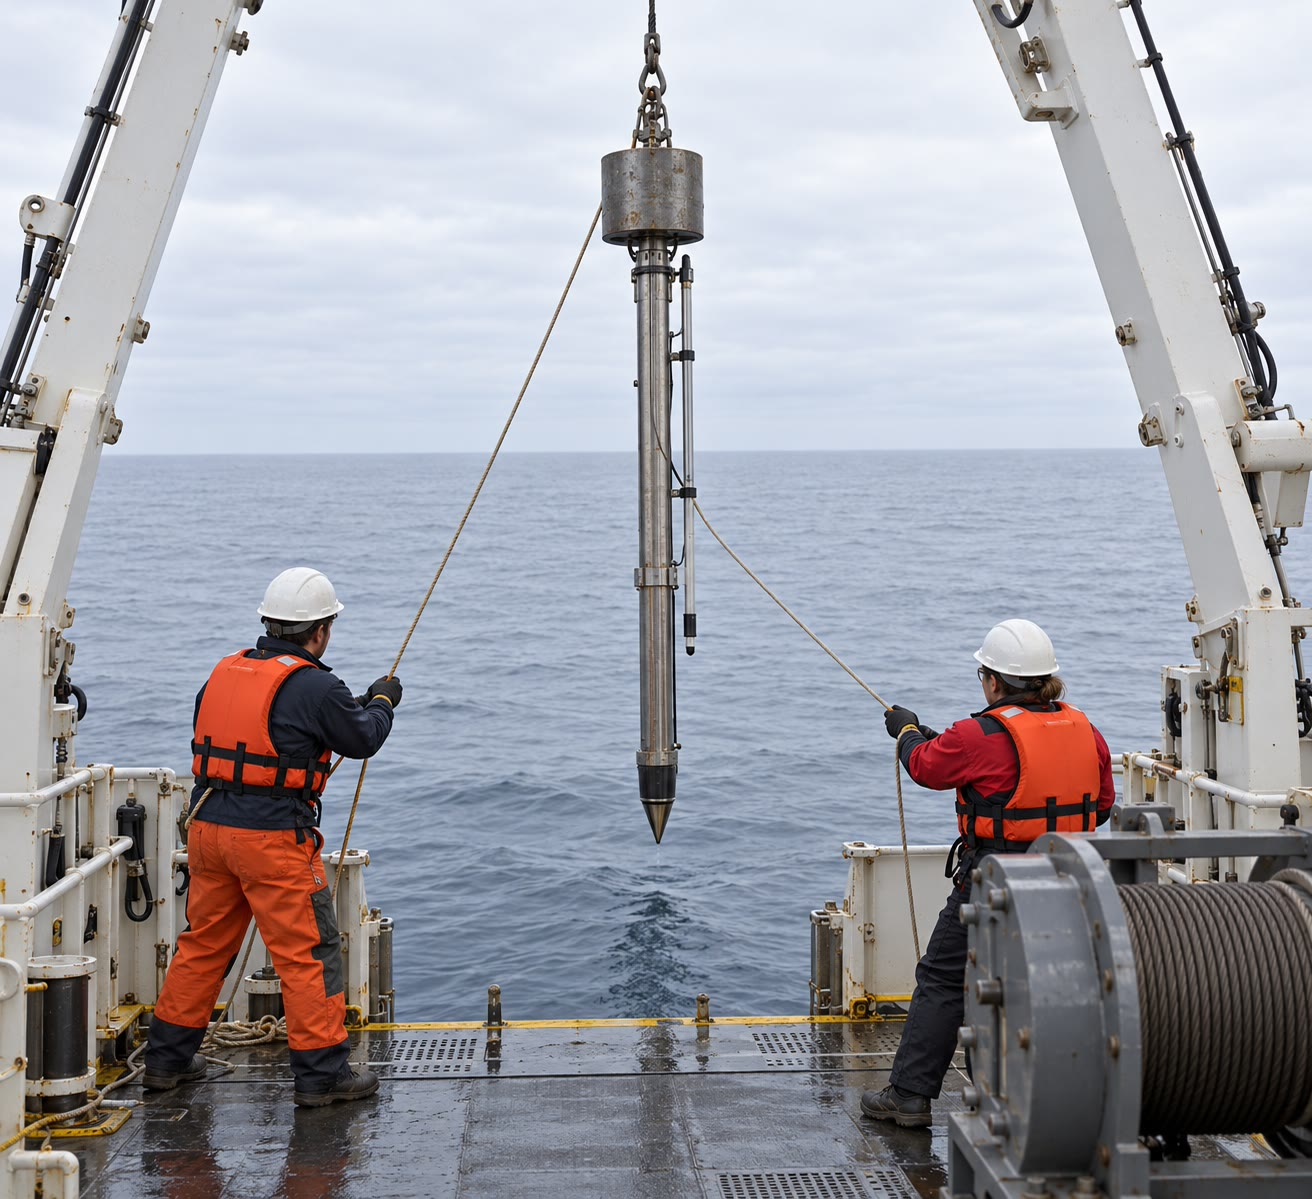
\includegraphics[width=\linewidth]{images/book5/ai/b3-heatflow-probe.jpg}

{\scriptsize A heat-flow lance about to be lowered from the stern of a
research ship (AI-generated illustration).}
\end{minipage}
\end{inthefield}

\section{Exercises}

\begin{exercise}[$\star$]\label{exo:b3:lithosphere-thermal-models:1}
With $\kappa = \qty{e-6}{m^2.s^{-1}}$, compute the conductive time $L^2/\kappa$
for $L = 1$, 10 and \qty{100}{km}, in millions of years.
\end{exercise}

\begin{exercise}[$\star$]\label{exo:b3:lithosphere-thermal-models:2}
A mountain range is eroded at \qty{1}{mm/yr}, and rock rises through the upper
\qty{30}{km} of crust to replace it. With $\kappa = \qty{e-6}{m^2.s^{-1}}$,
compute the Péclet number. Can the geotherm of the range be computed by
conduction alone?
\end{exercise}

\begin{exercise}[$\star$]\label{exo:b3:lithosphere-thermal-models:3}
In the half-space model ($T_0 = 0$, $T_m = \qty{1450}{\celsius}$, $\kappa =
\qty{0.8e-6}{m^2.s^{-1}}$), compute the temperature \qty{10}{km} below sea
floor \qty{5}{Myr} old (\qty{1}{Myr} $= \qty{3.156e13}{s}$; $\operatorname{erf}
0.445 = 0.471$).
\end{exercise}

\begin{exercise}[$\star$]\label{exo:b3:lithosphere-thermal-models:4}
With $C_q = \qty{490}{mW.m^{-2}.Myr^{1/2}}$, compute the heat flow through
sea floor 1, 25 and \qty{100}{Myr} old. Which of the three would a probe most
likely underestimate?
\end{exercise}

\begin{exercise}[$\star\star$]\label{exo:b3:lithosphere-thermal-models:5}
In the half-space model, the temperature reaches \qty{90}{\percent} of $T_m$
where $\operatorname{erf}\eta = 0.9$, $\eta = 1.163$. With $\kappa =
\qty{0.8e-6}{m^2.s^{-1}}$, compute that depth at 10, 40 and \qty{100}{Myr}.
\end{exercise}

\begin{exercise}[$\star\star$]\label{exo:b3:lithosphere-thermal-models:6}
With the values of the text, the half-space model gives $C =
\qty{370.5}{m.Myr^{-1/2}}$. Keeping every other value, what thermal expansion
coefficient would give the fitted \qty{350}{m.Myr^{-1/2}}? What other parameter
could be changed instead?
\end{exercise}

\begin{exercise}[$\star\star$]\label{exo:b3:lithosphere-thermal-models:7}
Compute the asymptotic heat flow $kT_m/L$ of the plate model for $L =
\qty{95}{km}$, $T_m = \qty{1450}{\celsius}$, and for $L = \qty{125}{km}$,
$T_m = \qty{1350}{\celsius}$, with $k = \qty{3.1}{W.m^{-1}.K^{-1}}$ in both.
Which is closer to the heat flow of old ocean floor computed from $C_q/\sqrt t$
at \qty{150}{Myr} with $C_q = \qty{490}{mW.m^{-2}.Myr^{1/2}}$?
\end{exercise}

\begin{exercise}[$\star\star$]\label{exo:b3:lithosphere-thermal-models:8}
A province has $q_0 = \qty{60}{mW.m^{-2}}$, $h_r = \qty{10}{km}$ and $A_0h_r =
0.4\,q_0$. Compute $A_0$, $q_m$ and the temperature at the Moho, \qty{35}{km}
deep, with $k = \qty{2.5}{W.m^{-1}.K^{-1}}$.
\end{exercise}

\begin{exercise}[$\star\star$]\label{exo:b3:lithosphere-thermal-models:9}
Two granite plutons of one province give $q_0 = \qty{66}{mW.m^{-2}}$ with $A_0
= \qty{3.0}{\micro W.m^{-3}}$, and $q_0 = \qty{48}{mW.m^{-2}}$ with $A_0 =
\qty{1.2}{\micro W.m^{-3}}$. Assuming they lie on the line of
\cref{prop:b3:lithosphere-thermal-models:exponential}, compute $h_r$ and $q_m$.
\end{exercise}

\begin{exercise}[$\star\star\star$]\label{exo:b3:lithosphere-thermal-models:10}
(a) Show that the heat lost through the sea floor between ages 0 and $t$, per
unit area, is $Q(t) = 2k(T_m - T_0)\sqrt{t/(\pi\kappa)}$ in the half-space
model. (b) Show that the subsidence is $d - d_r = \alpha Q/\bigl(c(\rho_m -
\rho_w)\bigr)$, where $c = k/(\rho_m\kappa)$ is the specific heat. (c) Check it
numerically at \qty{40}{Myr} with the values of the text.
\end{exercise}

\begin{exercise}[$\star\star\star$]\label{exo:b3:lithosphere-thermal-models:11}
In the plate model of the text ($\tau = \qty{36.2}{Myr}$, $\rho_m\alpha T_mL/
\bigl(2(\rho_m - \rho_w)\bigr) = \qty{3104}{m}$), the depth computed with the
first Fourier term alone exceeds the full series mainly by the $n = 3$ term.
Compute that term's size at 1, 10 and \qty{20}{Myr}, and the age after which
the first term alone is within \qty{10}{m} of the series.
\end{exercise}

\begin{exercise}[$\star\star\star$]\label{exo:b3:lithosphere-thermal-models:12}
(a) Show that, in the geotherm of \cref{prop:b3:lithosphere-thermal-models:exponential},
$T(z) \approx q_mz/k + A_0h_r^2/k$ for $z \gg h_r$. (b) Deduce the depth of the
\qty{1300}{\celsius} isotherm for $q_0 = \qty{40}{mW.m^{-2}}$, with the values
of exercise 8. (c) By how much must $q_m$ fall for that depth to reach
\qty{250}{km}, the depth of the fast roots of cratons?
\end{exercise}

\section{Problem: Forty Million Years off the Ridge}

\begin{problem}[{Weekend problem --- the half-space and the plate, the depth of
an invented ocean, and the thickness of its plate}]
\label{pb:b3:lithosphere-thermal-models:1}
% values: calc/ch05.py; plate_cooling.py; honda04:gdh1, ps77:depth-age, data:b5-depth-age
Take $T_0 = 0$, $T_m = \qty{1450}{\celsius}$, $\kappa =
\qty{0.8e-6}{m^2.s^{-1}}$, $k = \qty{3.1}{W.m^{-1}.K^{-1}}$, $\alpha =
\qty{3.1e-5}{K^{-1}}$, $\rho_m = \qty{3300}{kg.m^{-3}}$, $\rho_w =
\qty{1030}{kg.m^{-3}}$, a ridge \qty{2500}{m} deep, and \qty{1}{Myr} $=
\qty{3.156e13}{s}$.

\medskip\noindent\textbf{Part I --- The half-space.}
\begin{enumerate}
  \item Compute $\sqrt{\kappa t}$ at 10 and \qty{40}{Myr}.
  \item Compute the temperature \qty{20}{km} below the floor at both ages
        ($\operatorname{erf}0.6294 = 0.6266$, $\operatorname{erf}0.3147 =
        0.3437$).
  \item The \qty{1000}{\celsius} isotherm lies where $\operatorname{erf}\eta =
        0.6897$, $\eta = 0.7174$. Compute its depth at both ages, and the age
        at which it reaches \qty{60}{km}.
  \item Compute the heat flow at both ages, and $C_q$.
  \item A ridge spreads at \qty{25}{mm/yr} on each side. Compute the Péclet
        number of the plate over \qty{95}{km}. Why may each column be cooled
        alone?
  \item Compute the conductive time across \qty{95}{km}. What does it say of
        a half-space model of floor \qty{150}{Myr} old?
\end{enumerate}

\medskip\noindent\textbf{Part II --- Subsidence.}
\begin{enumerate}[resume]
  \item Recall the isostatic balance that turns the temperature deficit of a
        column into subsidence, and why the integral may be taken to infinity
        in the half-space.
  \item Compute $C$ of the depth--age law, and the depths at 10 and
        \qty{40}{Myr}.
  \item The median depth of the real ocean floor between 40 and \qty{45}{Myr}
        is \qty{4475}{m}, uncorrected. Compare with the model at
        \qty{42.5}{Myr}, and list what the median includes that the model
        leaves out.
  \item By how much would $C$ change if $T_m$ were \qty{1350}{\celsius}?
        Compare with the fitted \qty{350}{m.Myr^{-1/2}}.
  \item Why do measured heat flows on young floor fall below $C_q/\sqrt t$?
\end{enumerate}

\medskip\noindent\textbf{Part III --- The plate.} Take $L = \qty{95}{km}$.
\begin{enumerate}[resume]
  \item Compute $\tau$ and the amplitude $\rho_m\alpha T_mL/\bigl(2(\rho_m -
        \rho_w)\bigr)$.
  \item Compute the depth at \qty{40}{Myr} with the terms $n = 1$, 3 and 5.
  \item How much does the first term alone differ from that, and why so
        little?
  \item Compute the difference between the half-space and the plate at 40 and
        \qty{50}{Myr}, and estimate by linear interpolation the age at which
        it reaches \qty{100}{m}.
  \item Compute the heat flow of the plate at \qty{40}{Myr}, with the terms
        $n = 1$ to 3, and compare with the half-space.
  \item Give the asymptotic depth and heat flow.
\end{enumerate}

\medskip\noindent\textbf{Part IV --- An invented ocean.} In an invented ocean
whose ridge is \qty{2500}{m} deep, the floor, once corrected for sediment
and away from seamounts and swells, is \qty{5700}{m} deep at \qty{120}{Myr} and
\qty{4800}{m} at \qty{40}{Myr}. The plate's $L$ is unknown; every other value
is as above.
\begin{enumerate}[resume]
  \item Keeping the first Fourier term only, write the depth at
        \qty{120}{Myr} as a function of $L$, with $\tau$ itself depending on
        $L$.
  \item Solve it for $L$ by iteration, starting from $L = \qty{100}{km}$:
        compute $\tau$, then the $L$ that matches \qty{5700}{m} with that
        $\tau$, and repeat.
  \item With the $L$ found, compute the depth at \qty{40}{Myr} and compare
        with the half-space and with the \qty{4800}{m} measured.
  \item Compute $\tau$ for that $L$ and the asymptotic depth of this ocean.
  \item After what age does the floor lie within \qty{100}{m} of its
        asymptotic depth?
  \item Give the thickness $L$ of the plate that fits the old floor of the
        invented ocean.
\end{enumerate}
\end{problem}
